% !TEX root = ../main.tex
%% ---------------------------------------------------------------------------
% 4.3 1D manufactured beam
%% ---------------------------------------------------------------------------

\subsection{1D manufactured beam}\label{sec:manufactured1d}

In order to assess the convergence performance of Galerkin meshfree methods with cubic and quartic basis function, we consider a manufactured beam as shown in Fig. \ref{fig:14}, and an octal polynomial solution is employed to perform the meshfree computation:
\begin{equation}\label{beam_manufactured}
w=x^{8}/100+2x^{7}/100+x^{6}+x^{5}+5x^{4}+3x^{3}+4x^{2}+5x+6
\end{equation}
All specific values of boundary conditions are determined by Eq. \eqref{beam_manufactured}.
The displacement and moment boundary conditions are imposed on both sides.
Also, the material and geometry properties are the same as 1D cantilever beam in Section \ref{sec:quadratic}.

\begin{figure}[pos=htbp]
\centering
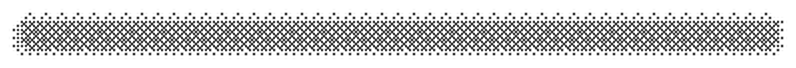
\includegraphics[width=0.85\textwidth]{figs/fig14.png}
\caption{Description of 1D manufactured beam.}\label{fig:14}
\end{figure}

Five meshfree discretizations with 11, 21, 41, 81, 161 nodes are adopted to observe the convergence performance.
For meshfree computation, the normalized support sizes are respectively prescribed as 3.5 and 4.5 for $p=3,4$.
The convergence results referring to $L_2$, $H_1$ and $H_2$ error norms for cubic and quartic meshfree formulation are listed in Figs. \ref{fig:15}--\ref{fig:20}, respectively.
The results clearly show that the convergence rates of GI-3, GI-6 and GI-9 adopted in cubic meshfree formulation, GI-4, GI-8 and GI-13 adopted in quartic meshfree formulation both are 2, 1, 0, respectively.
This is because Gauss integration can not meet the cubic and quartic integration constraints corresponding to the orders of basis functions, i.e., the integration consistency of GI is $q=1$, which is lower than $p$, thus the integration error totally governs the convergence performance of Galerkin meshfree methods with the nodal distance constantly decreasing.
On the contrary, according to the previous description, since RKGSI based meshfree formulation possess corresponding integration consistency $q=p$, it is capable for producing optimal convergence rates of $L_2$, $H_1$ and $H_2$ error norms, which respectively are 4, 3 and 2 in cubic case, 5, 4, 3 in quartic case.

\begin{figure}[pos=htbp]
\centering
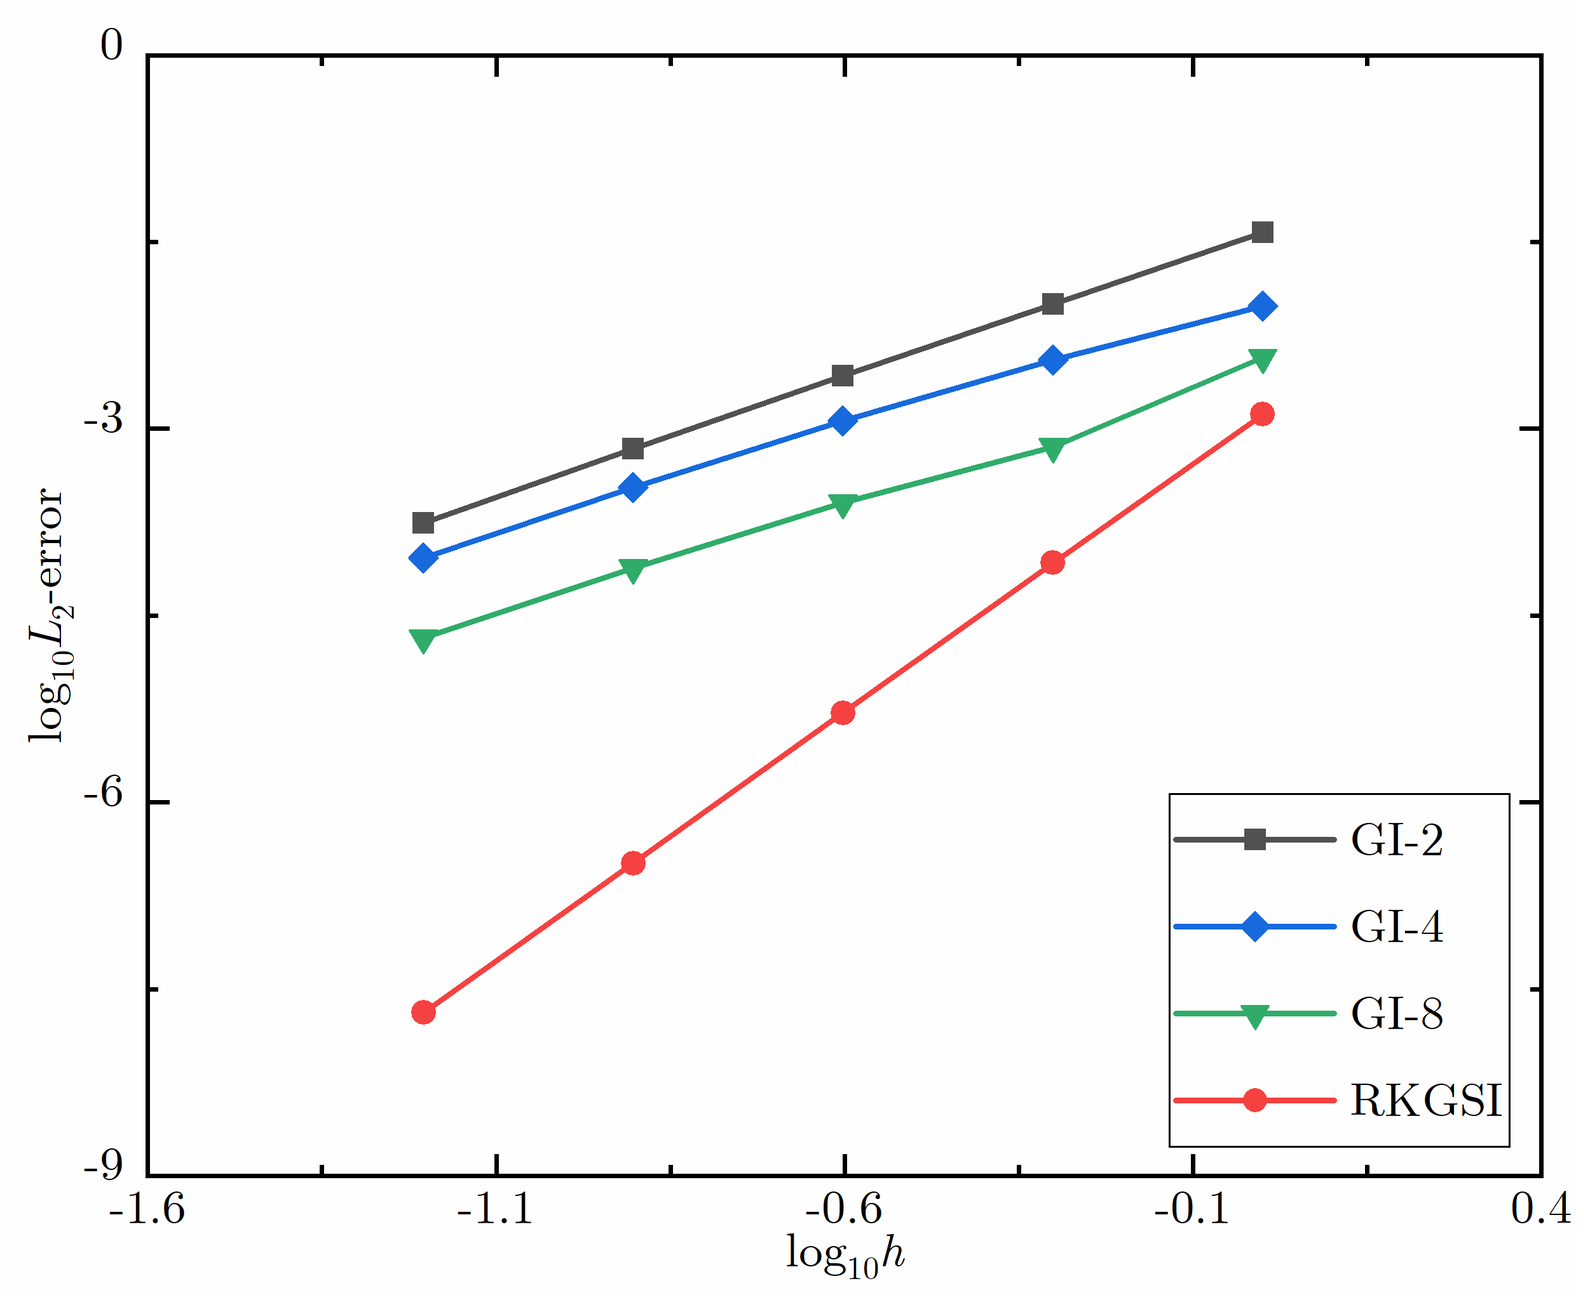
\includegraphics[width=0.55\textwidth]{figs/fig15.png}
\caption{$L_2$-error comparison for the 1D manufactured beam with $p=3$.}\label{fig:15}
\end{figure}

\begin{figure}[pos=htbp]
\centering
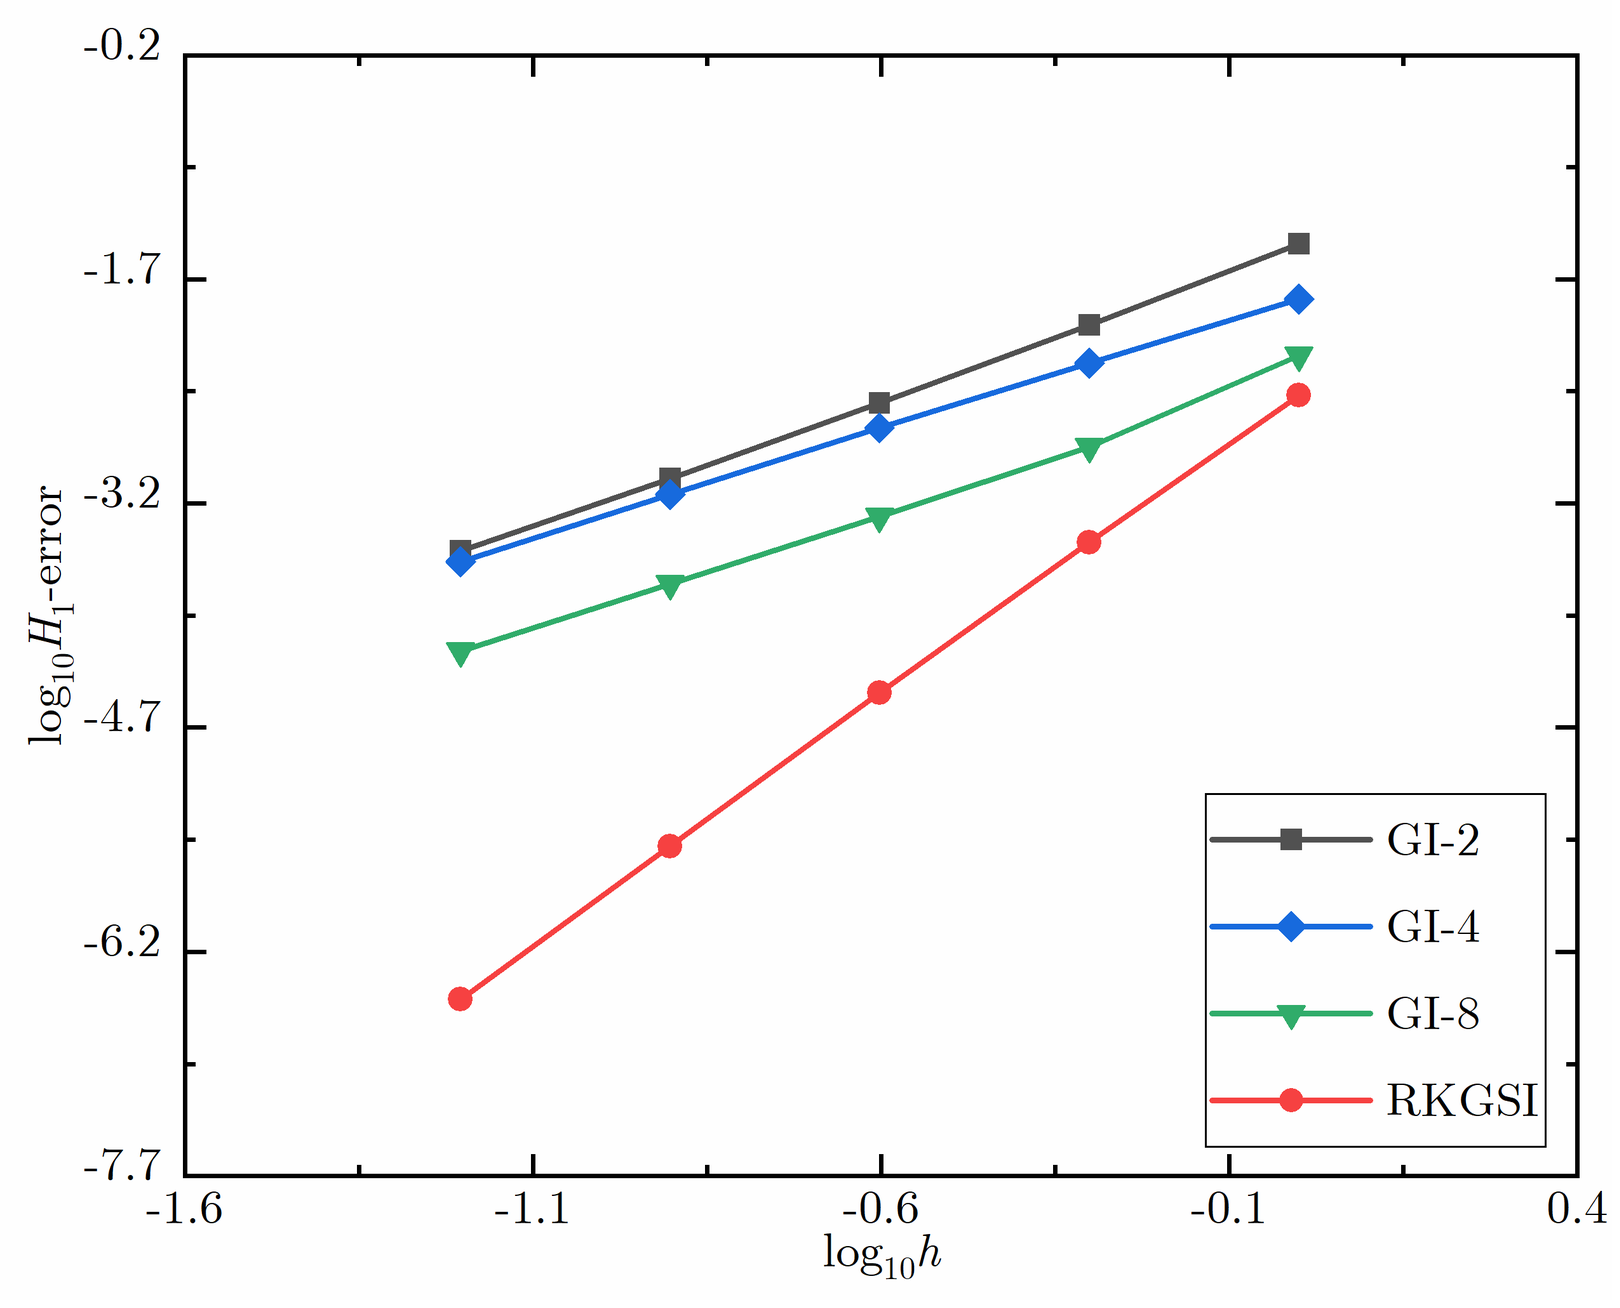
\includegraphics[width=0.55\textwidth]{figs/fig16.png}
\caption{$H_1$-error comparison for the 1D manufactured beam with $p=3$.}\label{fig:16}
\end{figure}

\begin{figure}[pos=htbp]
\centering
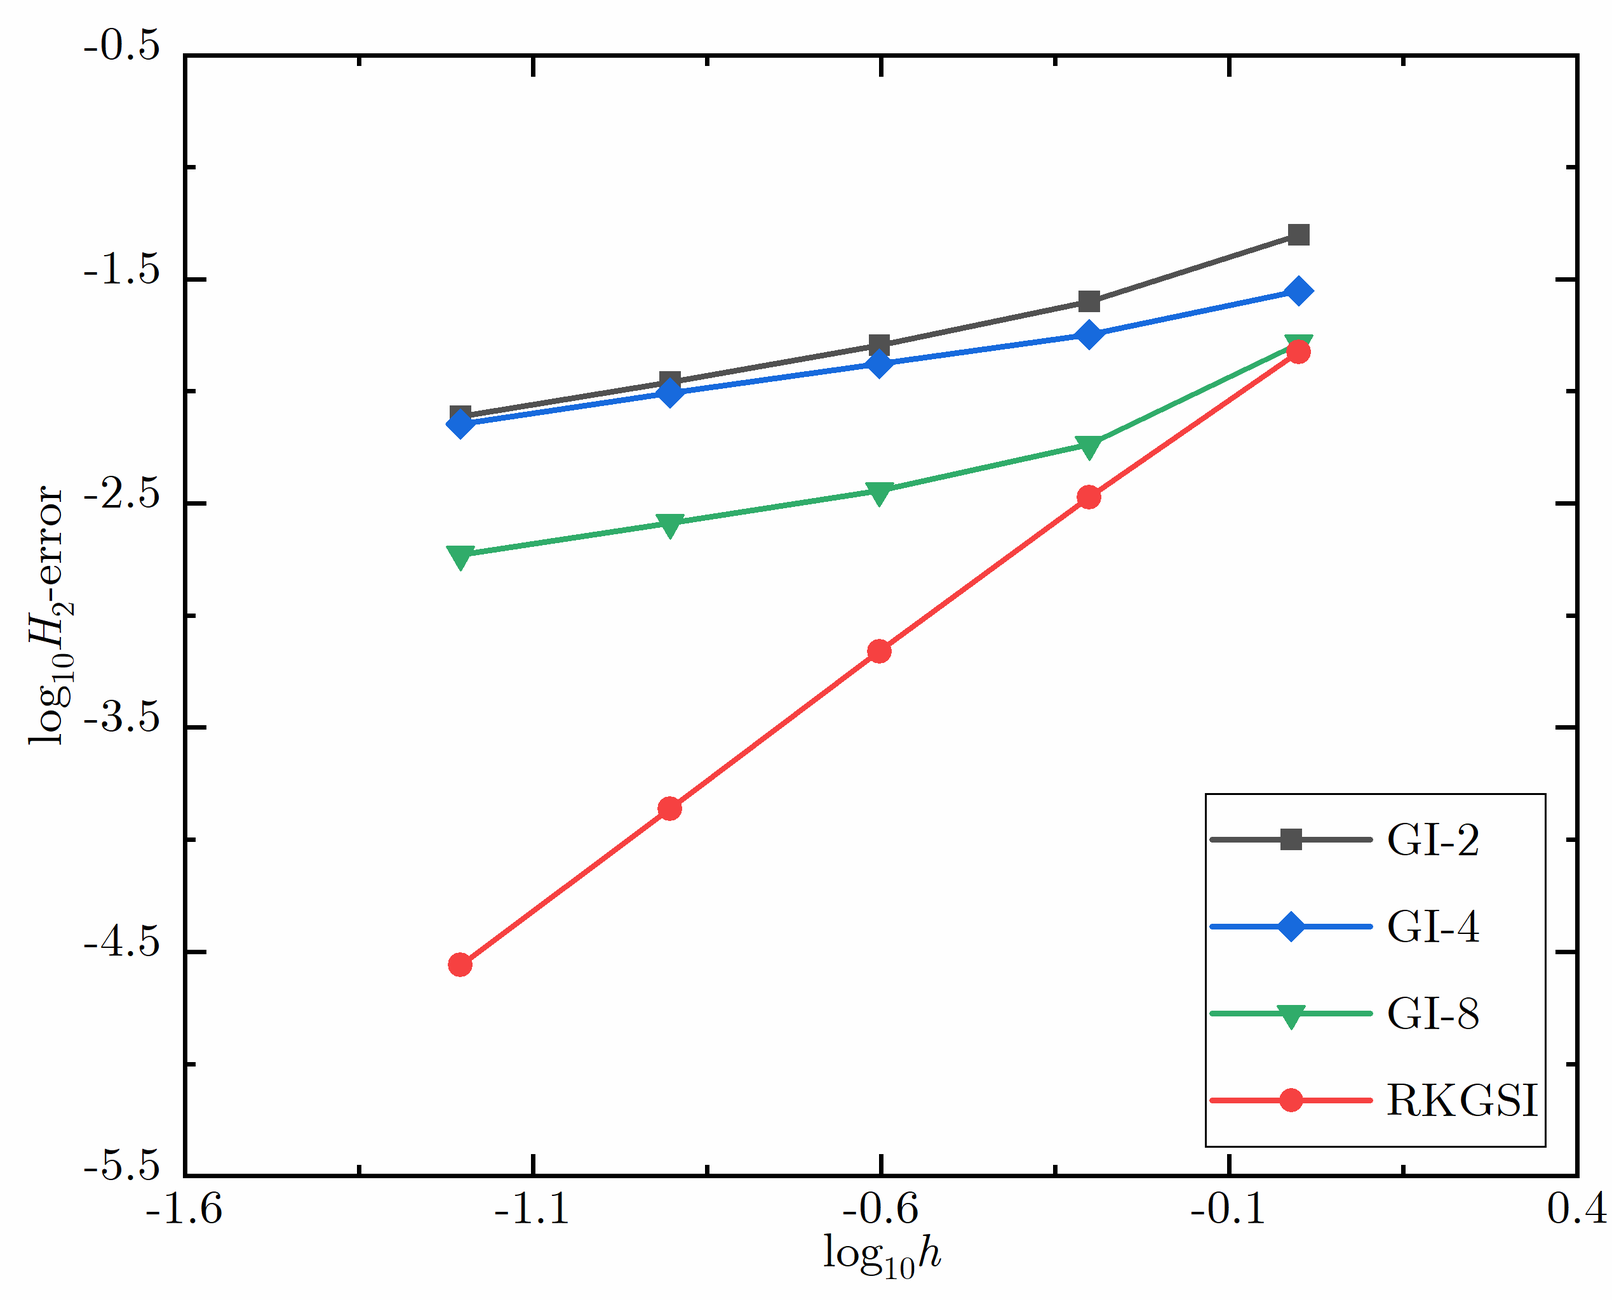
\includegraphics[width=0.55\textwidth]{figs/fig17.png}
\caption{$H_2$-error comparison for the 1D manufactured beam with $p=3$.}\label{fig:17}
\end{figure}

\begin{figure}[pos=htbp]
\centering
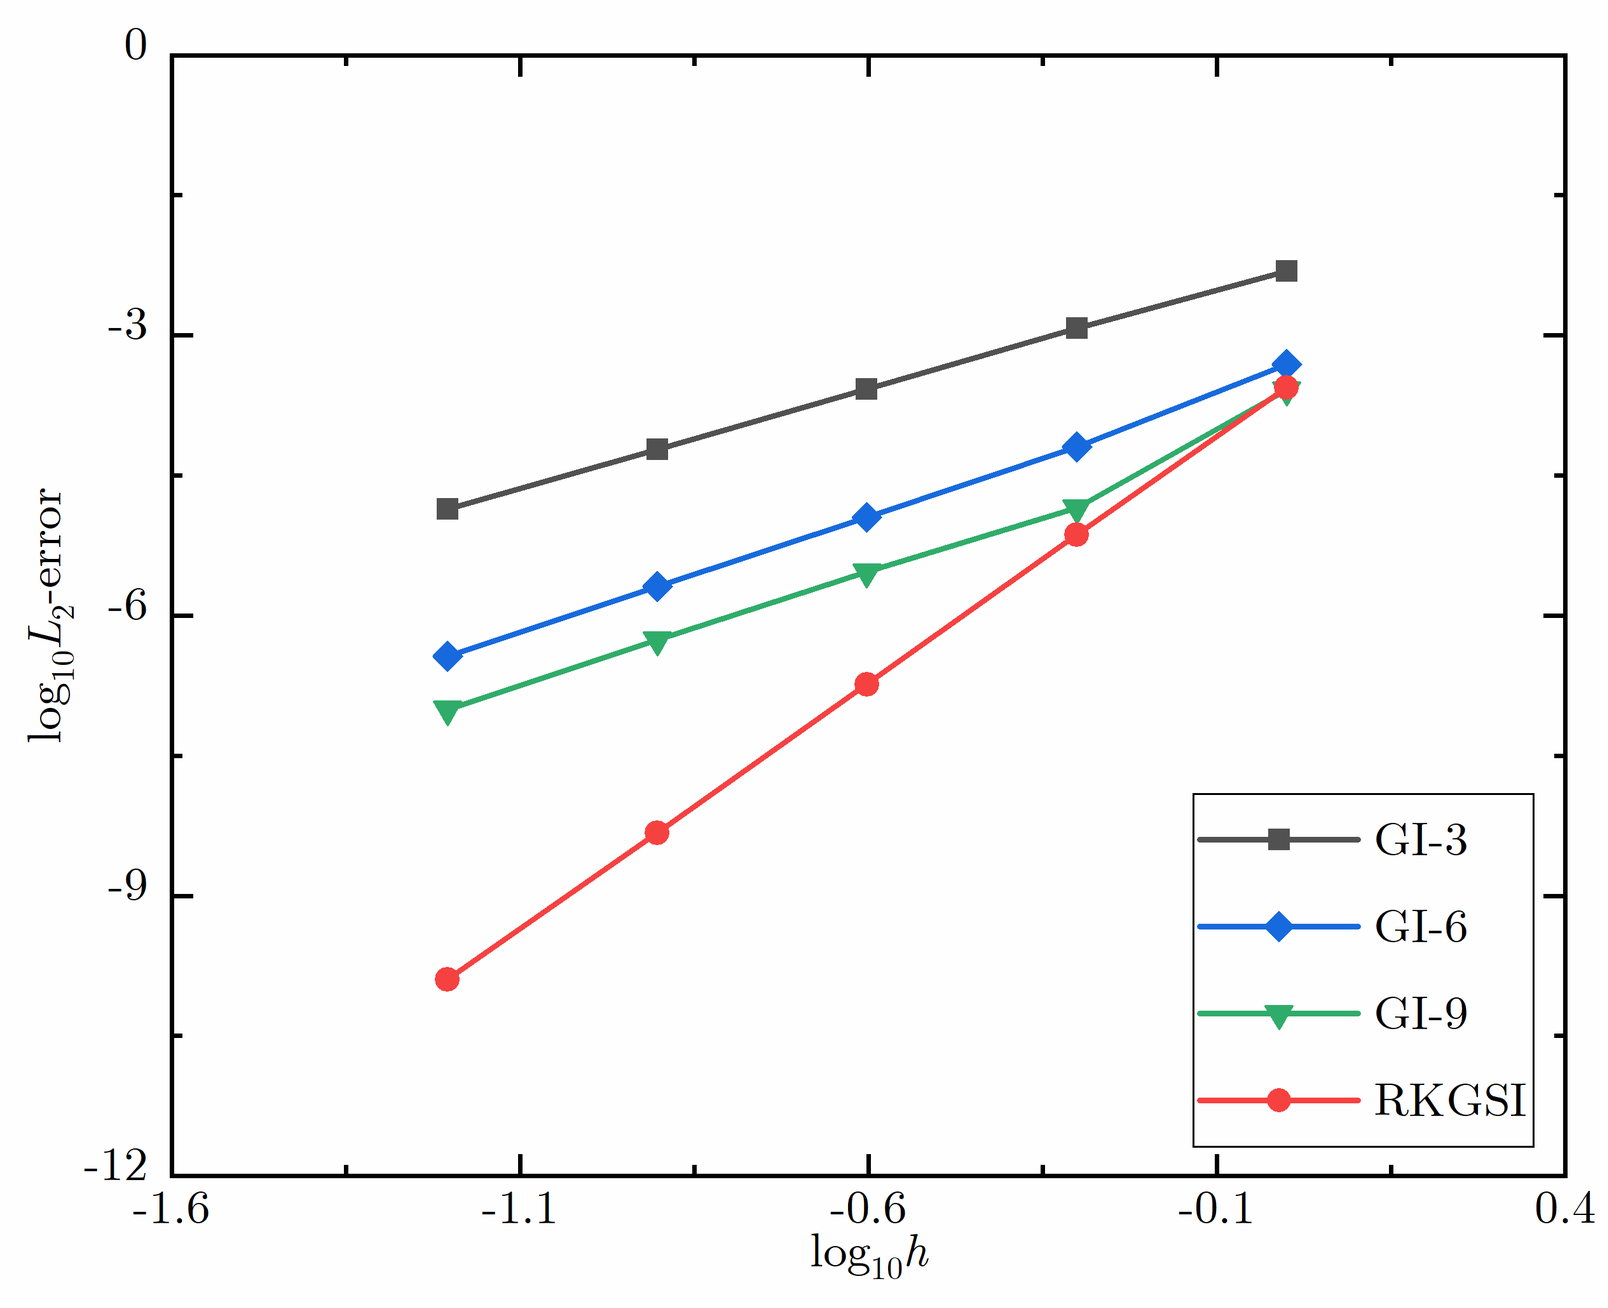
\includegraphics[width=0.55\textwidth]{figs/fig18.png}
\caption{$L_2$-error comparison for the 1D manufactured beam with $p=4$.}\label{fig:18}
\end{figure}

\begin{figure}[pos=htbp]
\centering
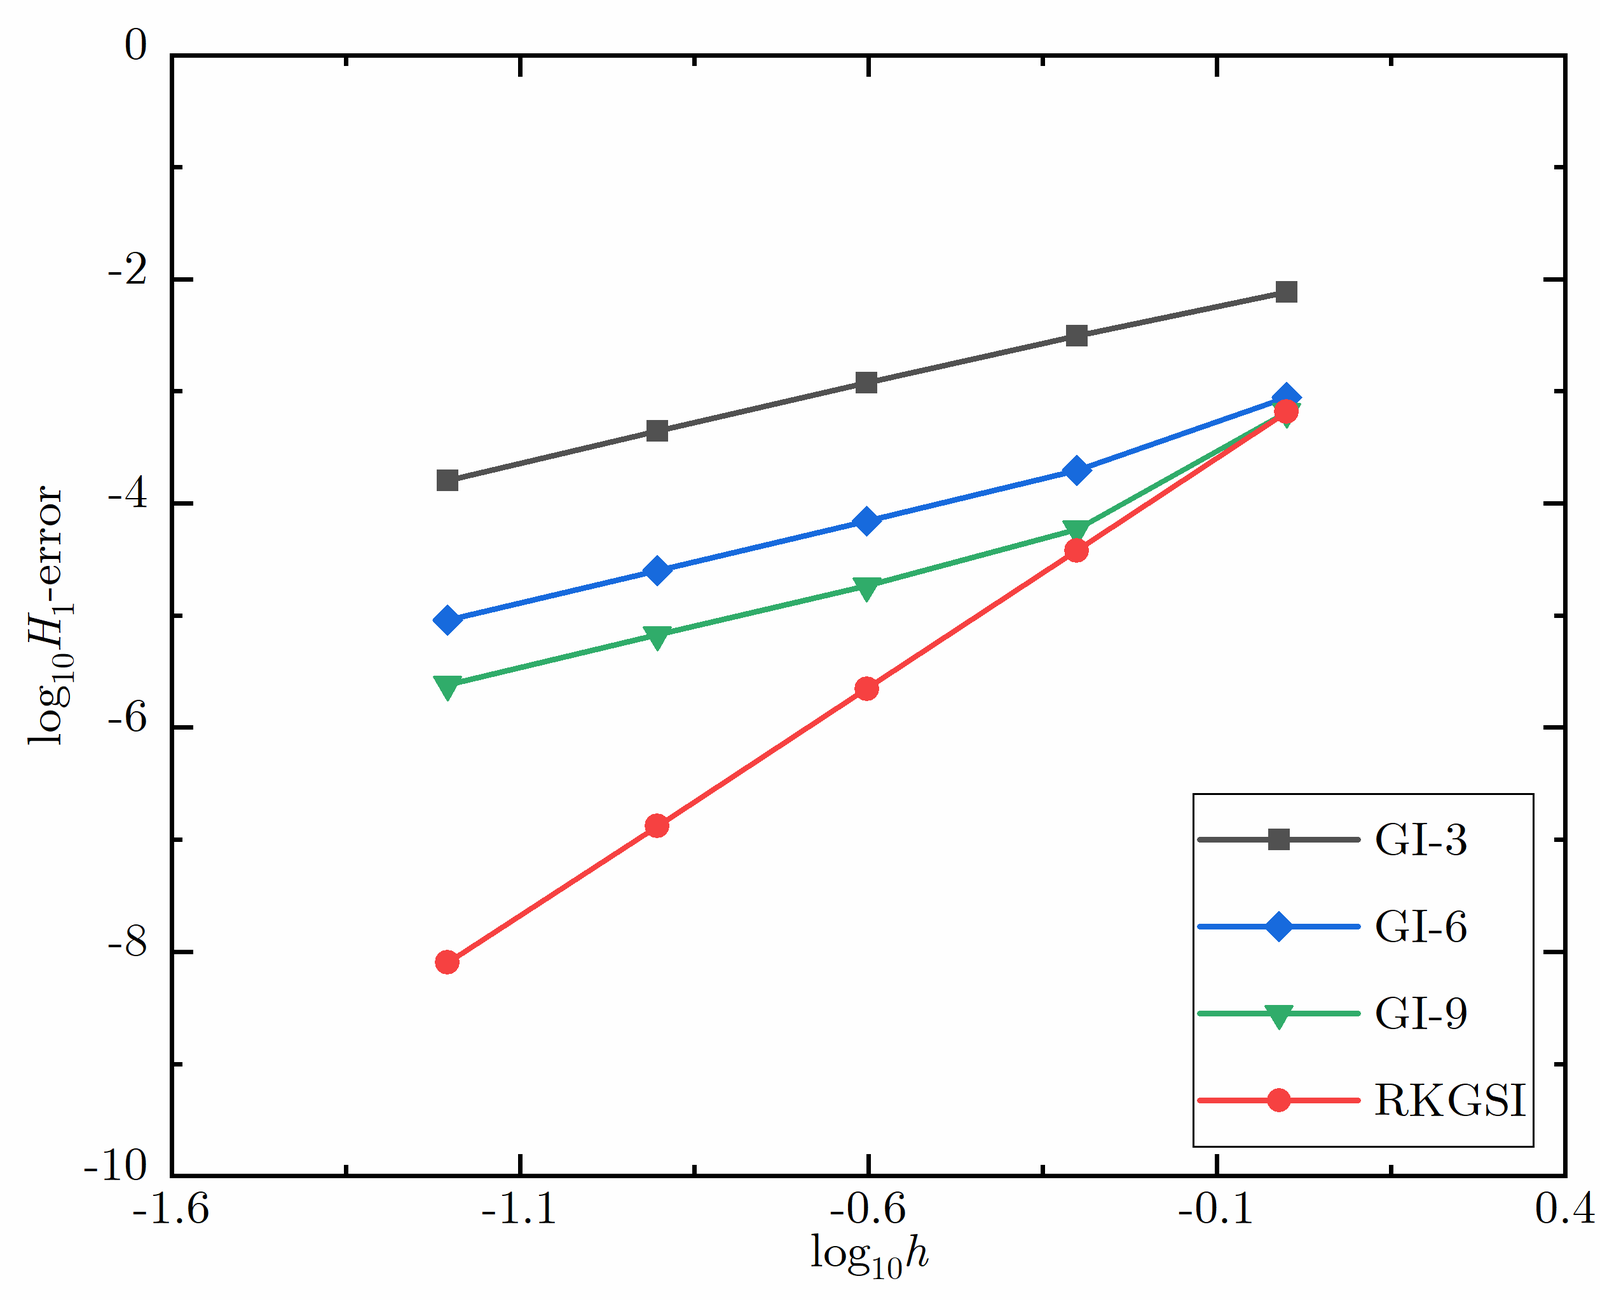
\includegraphics[width=0.55\textwidth]{figs/fig19.png}
\caption{$H_1$-error comparison for the 1D manufactured beam with $p=4$.}\label{fig:19}
\end{figure}

\begin{figure}[pos=htbp]
\centering
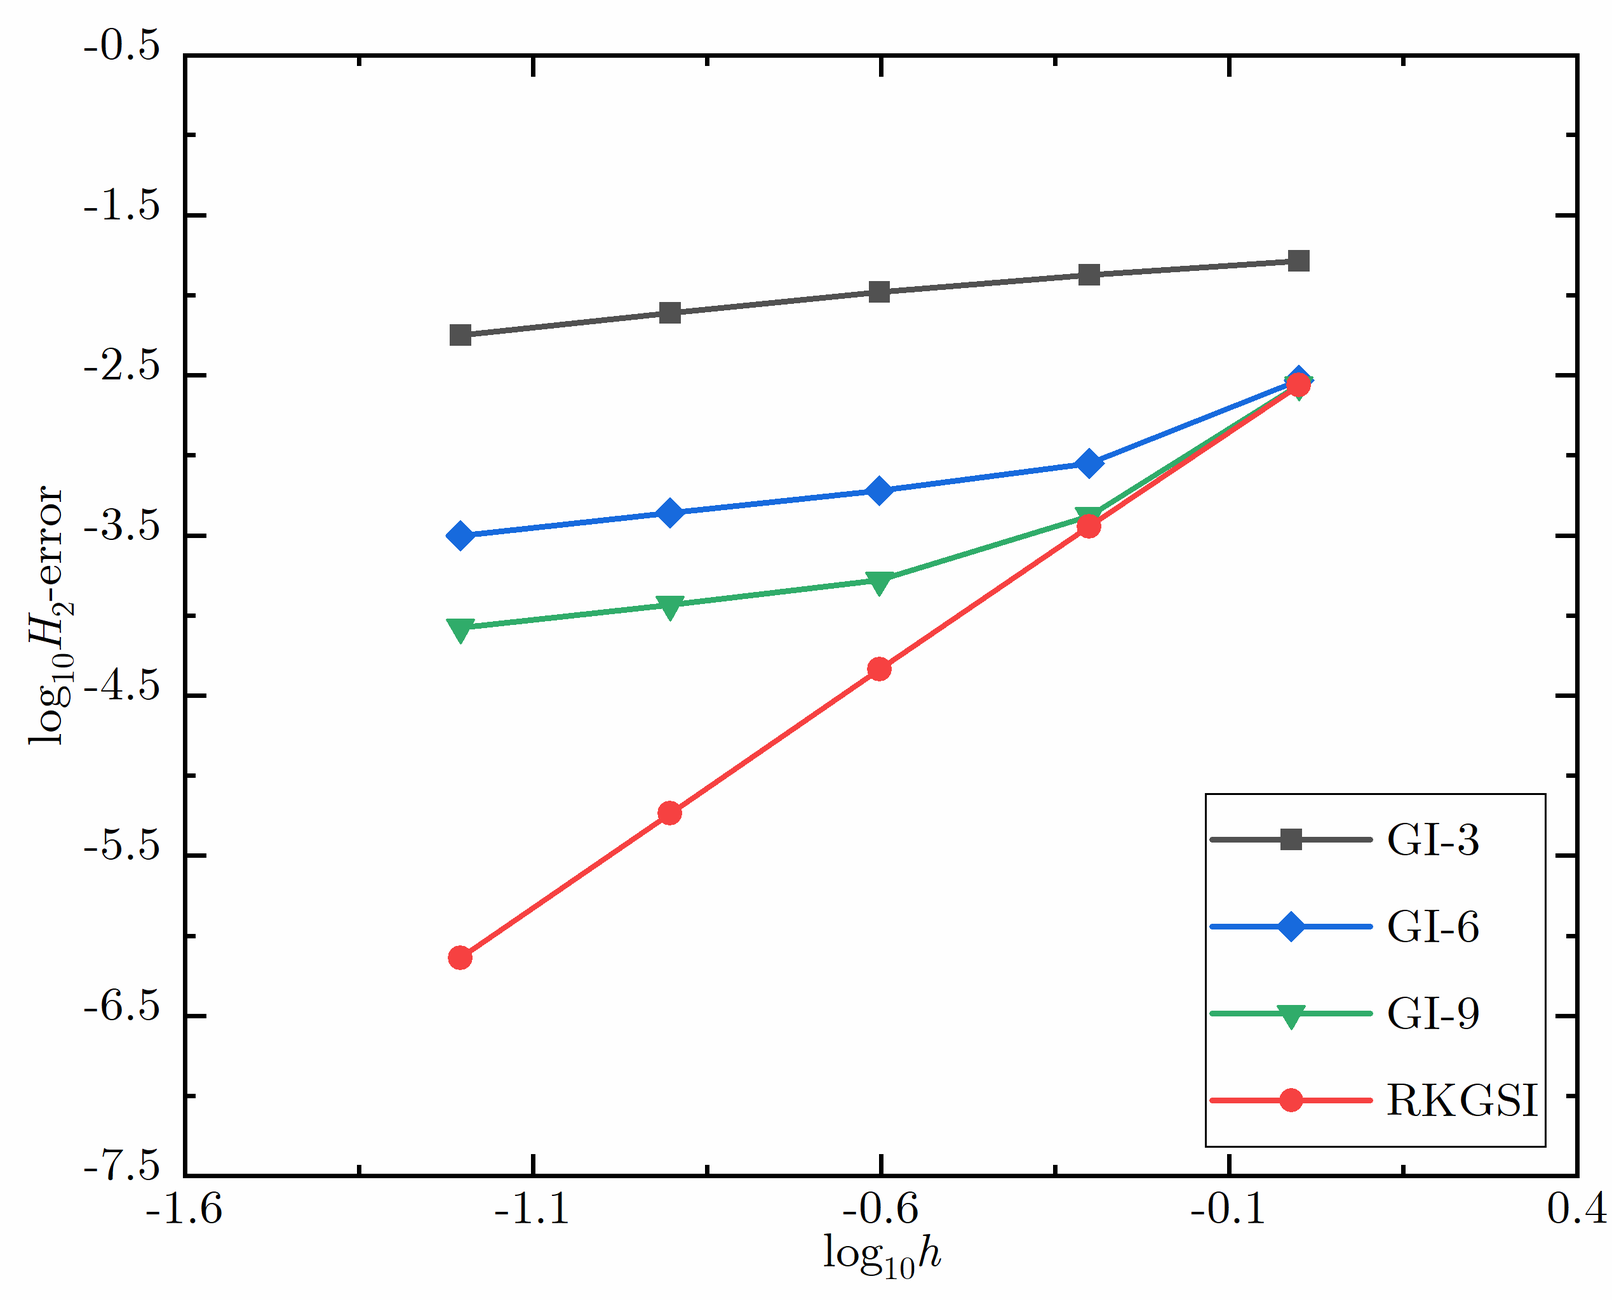
\includegraphics[width=0.55\textwidth]{figs/fig20.png}
\caption{$H_2$-error comparison for the 1D manufactured beam with $p=4$.}\label{fig:20}
\end{figure}
